\chapter{Evaluation and project planning} \label{chap:evalProjPlan}

This milestone will focus on planning development steps and guidelines based on the evaluation of the previous milestone (see \ref{chap:proofConcept}).
A concrete plan will help develop a maintainable, quality application with a clear vision of the target goal.

\section{Evaluation}

\subsection{Project hosting platform}

The resulting project shall be open source and will be hosted on GitHub.
These decisions were made to allow external contributions, reach a niche target demographic, and to have access to freemium tools, which are offered for free to open source projects.

GitHub was chosen over GitLab, the second best contendor, because the former platform offers better visibility and access - a crucial factor for reaching the target demographic.

\subsection{Technology stack}

The proof of concept application (see \ref{chap:proofConcept}) was developed in November 2018 using \nameref{sec:netFramework} and is hosted on GitLab\footnote{https://gitlab.com/hailstorm75/markdoc}. The resulting project shall be developed using \nameref{sec:netCore}, as it is the new development platform from Microsoft (see \ref{chap:overviewNET}). There are no reasons to stick with the old development platform, only drawbacks.

C\# will be the primary programming language, as it is the dominant language for the \ref{gloss:dotnetlabel} platform.
F\# shall be used sparsly to fullfill a personal goal of exploring said languages capabilities.

\section{Development planning}

\subsection{Project architecture}



\tikzset{every picture/.style={line width=0.75pt}} %set default line width to 0.75pt

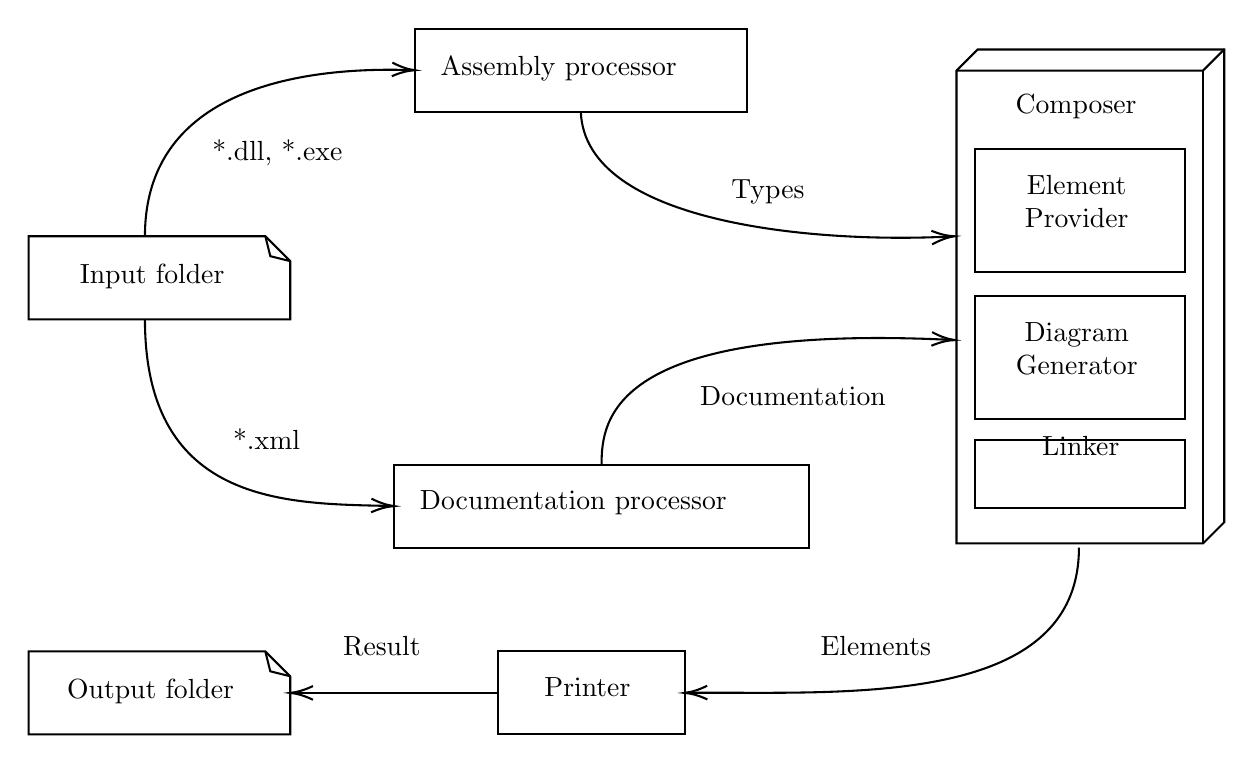
\begin{tikzpicture}[x=0.75pt,y=0.75pt,yscale=-1,xscale=1]
%uncomment if require: \path (0,428); %set diagram left start at 0, and has height of 428

%Shape: Folded Corner [id:dp38453805550218356] 
\draw   (128,110) -- (14,110) -- (14,150) -- (140,150) -- (140,122) -- cycle -- (128,110) ; \draw   (140,122) -- (130.4,119.6) -- (128,110) ;

%Shape: Cube [id:dp9514351083967096] 
\draw   (461,30.21) -- (471.21,20) -- (590,20) -- (590,247.79) -- (579.79,258) -- (461,258) -- cycle ; \draw   (590,20) -- (579.79,30.21) -- (461,30.21) ; \draw   (579.79,30.21) -- (579.79,258) ;
%Shape: Rectangle [id:dp28951515389797833] 
\draw   (470,68) -- (571,68) -- (571,127) -- (470,127) -- cycle ;

%Shape: Rectangle [id:dp811482931901953] 
\draw   (470,208) -- (571,208) -- (571,241) -- (470,241) -- cycle ;

%Shape: Rectangle [id:dp5590157968822316] 
\draw   (470,139) -- (571,139) -- (571,198) -- (470,198) -- cycle ;


%Shape: Rectangle [id:dp0837615901192712] 
\draw   (200,10) -- (360,10) -- (360,50) -- (200,50) -- cycle ;

%Shape: Rectangle [id:dp21181013544630467] 
\draw   (190,220) -- (390,220) -- (390,260) -- (190,260) -- cycle ;

%Curve Lines [id:da5699658849973097] 
\draw    (70,110) .. controls (70,31.86) and (161.2,28.74) .. (198.34,29.94) ;
\draw [shift={(200,30)}, rotate = 182.12] [color={rgb, 255:red, 0; green, 0; blue, 0 }  ][line width=0.75]    (10.93,-3.29) .. controls (6.95,-1.4) and (3.31,-0.3) .. (0,0) .. controls (3.31,0.3) and (6.95,1.4) .. (10.93,3.29)   ;
%Curve Lines [id:da0934002278421866] 
\draw    (70,150) .. controls (70,240.75) and (140.57,238.72) .. (188.55,239.96) ;
\draw [shift={(190,240)}, rotate = 181.59] [color={rgb, 255:red, 0; green, 0; blue, 0 }  ][line width=0.75]    (10.93,-3.29) .. controls (6.95,-1.4) and (3.31,-0.3) .. (0,0) .. controls (3.31,0.3) and (6.95,1.4) .. (10.93,3.29)   ;
%Curve Lines [id:da9139301607505403] 
\draw    (280,50) .. controls (281.98,104.12) and (393.73,113.48) .. (458.07,110.11) ;
\draw [shift={(460,110)}, rotate = 176.72] [color={rgb, 255:red, 0; green, 0; blue, 0 }  ][line width=0.75]    (10.93,-3.29) .. controls (6.95,-1.4) and (3.31,-0.3) .. (0,0) .. controls (3.31,0.3) and (6.95,1.4) .. (10.93,3.29)   ;
%Curve Lines [id:da360087403261089] 
\draw    (290,220) .. controls (290,198.67) and (294,151.67) .. (460,160) ;
\draw [shift={(460,160)}, rotate = 182.87] [color={rgb, 255:red, 0; green, 0; blue, 0 }  ][line width=0.75]    (10.93,-3.29) .. controls (6.95,-1.4) and (3.31,-0.3) .. (0,0) .. controls (3.31,0.3) and (6.95,1.4) .. (10.93,3.29)   ;
%Shape: Rectangle [id:dp5335135464926624] 
\draw   (240,310) -- (330,310) -- (330,350) -- (240,350) -- cycle ;

%Curve Lines [id:da34448081447371903] 
\draw    (520,260) .. controls (520,338.61) and (403.18,329.1) .. (331.08,329.99) ;
\draw [shift={(330,330)}, rotate = 359.2] [color={rgb, 255:red, 0; green, 0; blue, 0 }  ][line width=0.75]    (10.93,-3.29) .. controls (6.95,-1.4) and (3.31,-0.3) .. (0,0) .. controls (3.31,0.3) and (6.95,1.4) .. (10.93,3.29)   ;
%Shape: Folded Corner [id:dp9495985347442353] 
\draw   (128,310) -- (14,310) -- (14,350) -- (140,350) -- (140,322) -- cycle -- (128,310) ; \draw   (140,322) -- (130.4,319.6) -- (128,310) ;
%Straight Lines [id:da8650986253114432] 
\draw    (240,330) -- (142,330) ;
\draw [shift={(140,330)}, rotate = 360] [color={rgb, 255:red, 0; green, 0; blue, 0 }  ][line width=0.75]    (10.93,-3.29) .. controls (6.95,-1.4) and (3.31,-0.3) .. (0,0) .. controls (3.31,0.3) and (6.95,1.4) .. (10.93,3.29)   ;

% Text Node
\draw (37.11,122) node [anchor=north west][inner sep=0.75pt]   [align=left] {Input folder};
% Text Node
\draw (485,79) node [anchor=north west][inner sep=0.75pt]   [align=left] {\begin{minipage}[lt]{48.65pt}\setlength\topsep{0pt}
\begin{center}
Element\\Provider
\end{center}

\end{minipage}};
% Text Node
\draw (499,205) node [anchor=north west][inner sep=0.75pt]   [align=left] {\begin{minipage}[lt]{30.51pt}\setlength\topsep{0pt}
\begin{center}
Linker
\end{center}

\end{minipage}};
% Text Node
\draw (485,150) node [anchor=north west][inner sep=0.75pt]   [align=left] {\begin{minipage}[lt]{48.65pt}\setlength\topsep{0pt}
\begin{center}
Diagram\\Generator
\end{center}

\end{minipage}};
% Text Node
\draw (488,40) node [anchor=north west][inner sep=0.75pt]   [align=left] {Composer};
% Text Node
\draw (211,22) node [anchor=north west][inner sep=0.75pt]   [align=left] {Assembly processor};
% Text Node
\draw (201,231) node [anchor=north west][inner sep=0.75pt]   [align=left] {Documentation processor};
% Text Node
\draw (101,62) node [anchor=north west][inner sep=0.75pt]   [align=left] {*.dll, *.exe};
% Text Node
\draw (111,201) node [anchor=north west][inner sep=0.75pt]   [align=left] {*.xml};
% Text Node
\draw (351,81) node [anchor=north west][inner sep=0.75pt]   [align=left] {Types};
% Text Node
\draw (336,181) node [anchor=north west][inner sep=0.75pt]   [align=left] {Documentation};
% Text Node
\draw (261,321) node [anchor=north west][inner sep=0.75pt]   [align=left] {Printer};
% Text Node
\draw (394,301) node [anchor=north west][inner sep=0.75pt]   [align=left] {Elements};
% Text Node
\draw (31,322) node [anchor=north west][inner sep=0.75pt]   [align=left] {Output folder};
% Text Node
\draw (164,301) node [anchor=north west][inner sep=0.75pt]   [align=left] {Result};


\end{tikzpicture}

